\chapter{Ideen und Konzepte}


% Hier geht es um die Fragestellung, wie Sie die formulierten Ziele der Arbeit erreichen wollen.
% Sie halten z.B. erste, grobe Ideen, skizzenhafte Lösungsansätze fest. Gibt es mehrere Wege, Ansätze
% um dieses Ziel zu erreichen, begründen Sie hier, warum Sie einen bestimmten Weg einschlagen.
% Beispiel für ein Softwareprojekt: Erste Gedanken über eine grobe Systemarchitektur. Ist z.B. eine
% Microservice-Architektur angebracht? Welche Alternativen bestehen, wo gibt es Problempunkte? Die
% Umsetzung, die Beurteilung der Machbarkeit und die detaillierte Beschreibung der umgesetzten
% Architektur sind dann Teil der Realisierung.
% Abgrenzung zu Kapitel 5:
% - Besteht ein wesentliches Projektziel darin, für Ihre Kunden z.B. ein Security-Konzept, ein
% Kommunikations-Konzeptes, ein IT-Fachkonzept oder ein anderes Fach-Konzept zu erstellen, dann
% wird die Entwicklung dieser (fachlichen) Konzepte unter «Realisierung» beschrieben (sie sind ja der
% eigentliche Kern Ihrer Arbeit).
% - Besteht z.B. ein wesentliches Ziel der Arbeit darin, eine passende Software-Architektur zu
% evaluieren, dann gehören die entsprechenden Beschreibungen ins Kapitel 5.


\section{Konfiguration}
\subsection{Motivation}
Bei der Landis+Gyr werden verschiedenen Stromzählermodelle entwickelt. Der DlmsQuickAccess soll mit möglichst allen kommunizieren können.
Wie bereits in XY TODO erwähnt, wird für die Kommunikation Code der ATS verwendet.
Damit dieser richtig funktionieren kann, werden folgende zwei Dateien benötigt:
- AddressList
- DLMS.xml
Für die Auflistung aller Objekte eines Zählers wird zusätzlich ein ObjectModel als XML Datei benötigt.
Diese drei Dateien unterscheiden sich von Produkt zu Produkt. Ebenfalls muss berücksichtigt werden, dass sich die Informationen in diesen Dateien jederzeit ändern können.
Insbesondere beim ObjectModel ist dies regelmässig der Fall.

Diese Konfigurationen sollen somit von den Produktteams verwaltet und versioniert werden können.

\subsection{Lösungsidee}
Eine Konfigurationsdatei in welcher die zuvor erwähnten Dateien definiert sind. Die soll im YAML format geschrieben sein, was das Bearbeiten vereinfacht.
Jedes Produktteam kann diese Konfigurationsdatei im Repository des Produktquellcodes ablegen und versionieren.

TODO
damit sich der DlmsQuickAccess beim Betriebssystem so registrieren kann, dass 
Diese Konfiurationsdateien sollen die Endung \".dlmsquickaccess\" tragen, 

Um das Wechseln zwischen Produkten zu vereinfachen, soll sich der DlmsQuickAccess zuvor verwendete Konfigurationen merken, so dass der Benutzer diese auswählen kann.


TODO ufschribe, was passiert bim erste start und bi doppelclick.



\section{Testkonzept}

Manuelle Testszenarien

\section{Model View ViewModel}\label{mvvm}

\section{Architektur}
Der Quellcode der Anwendung ist in mehrere C\# Projekte aufgeteilt.

Dies soll die Wiederverwendbarkeit der Komponenten sicherstellen.
Wenn in Zukunft eine Komponente wie bspw. die Kommunikation ausgetauscht werden soll, so müssen nur in einem spezifischen Teil des Codes Änderungen vorgenommen werden.

\begin{figure}[H]
   \centering
   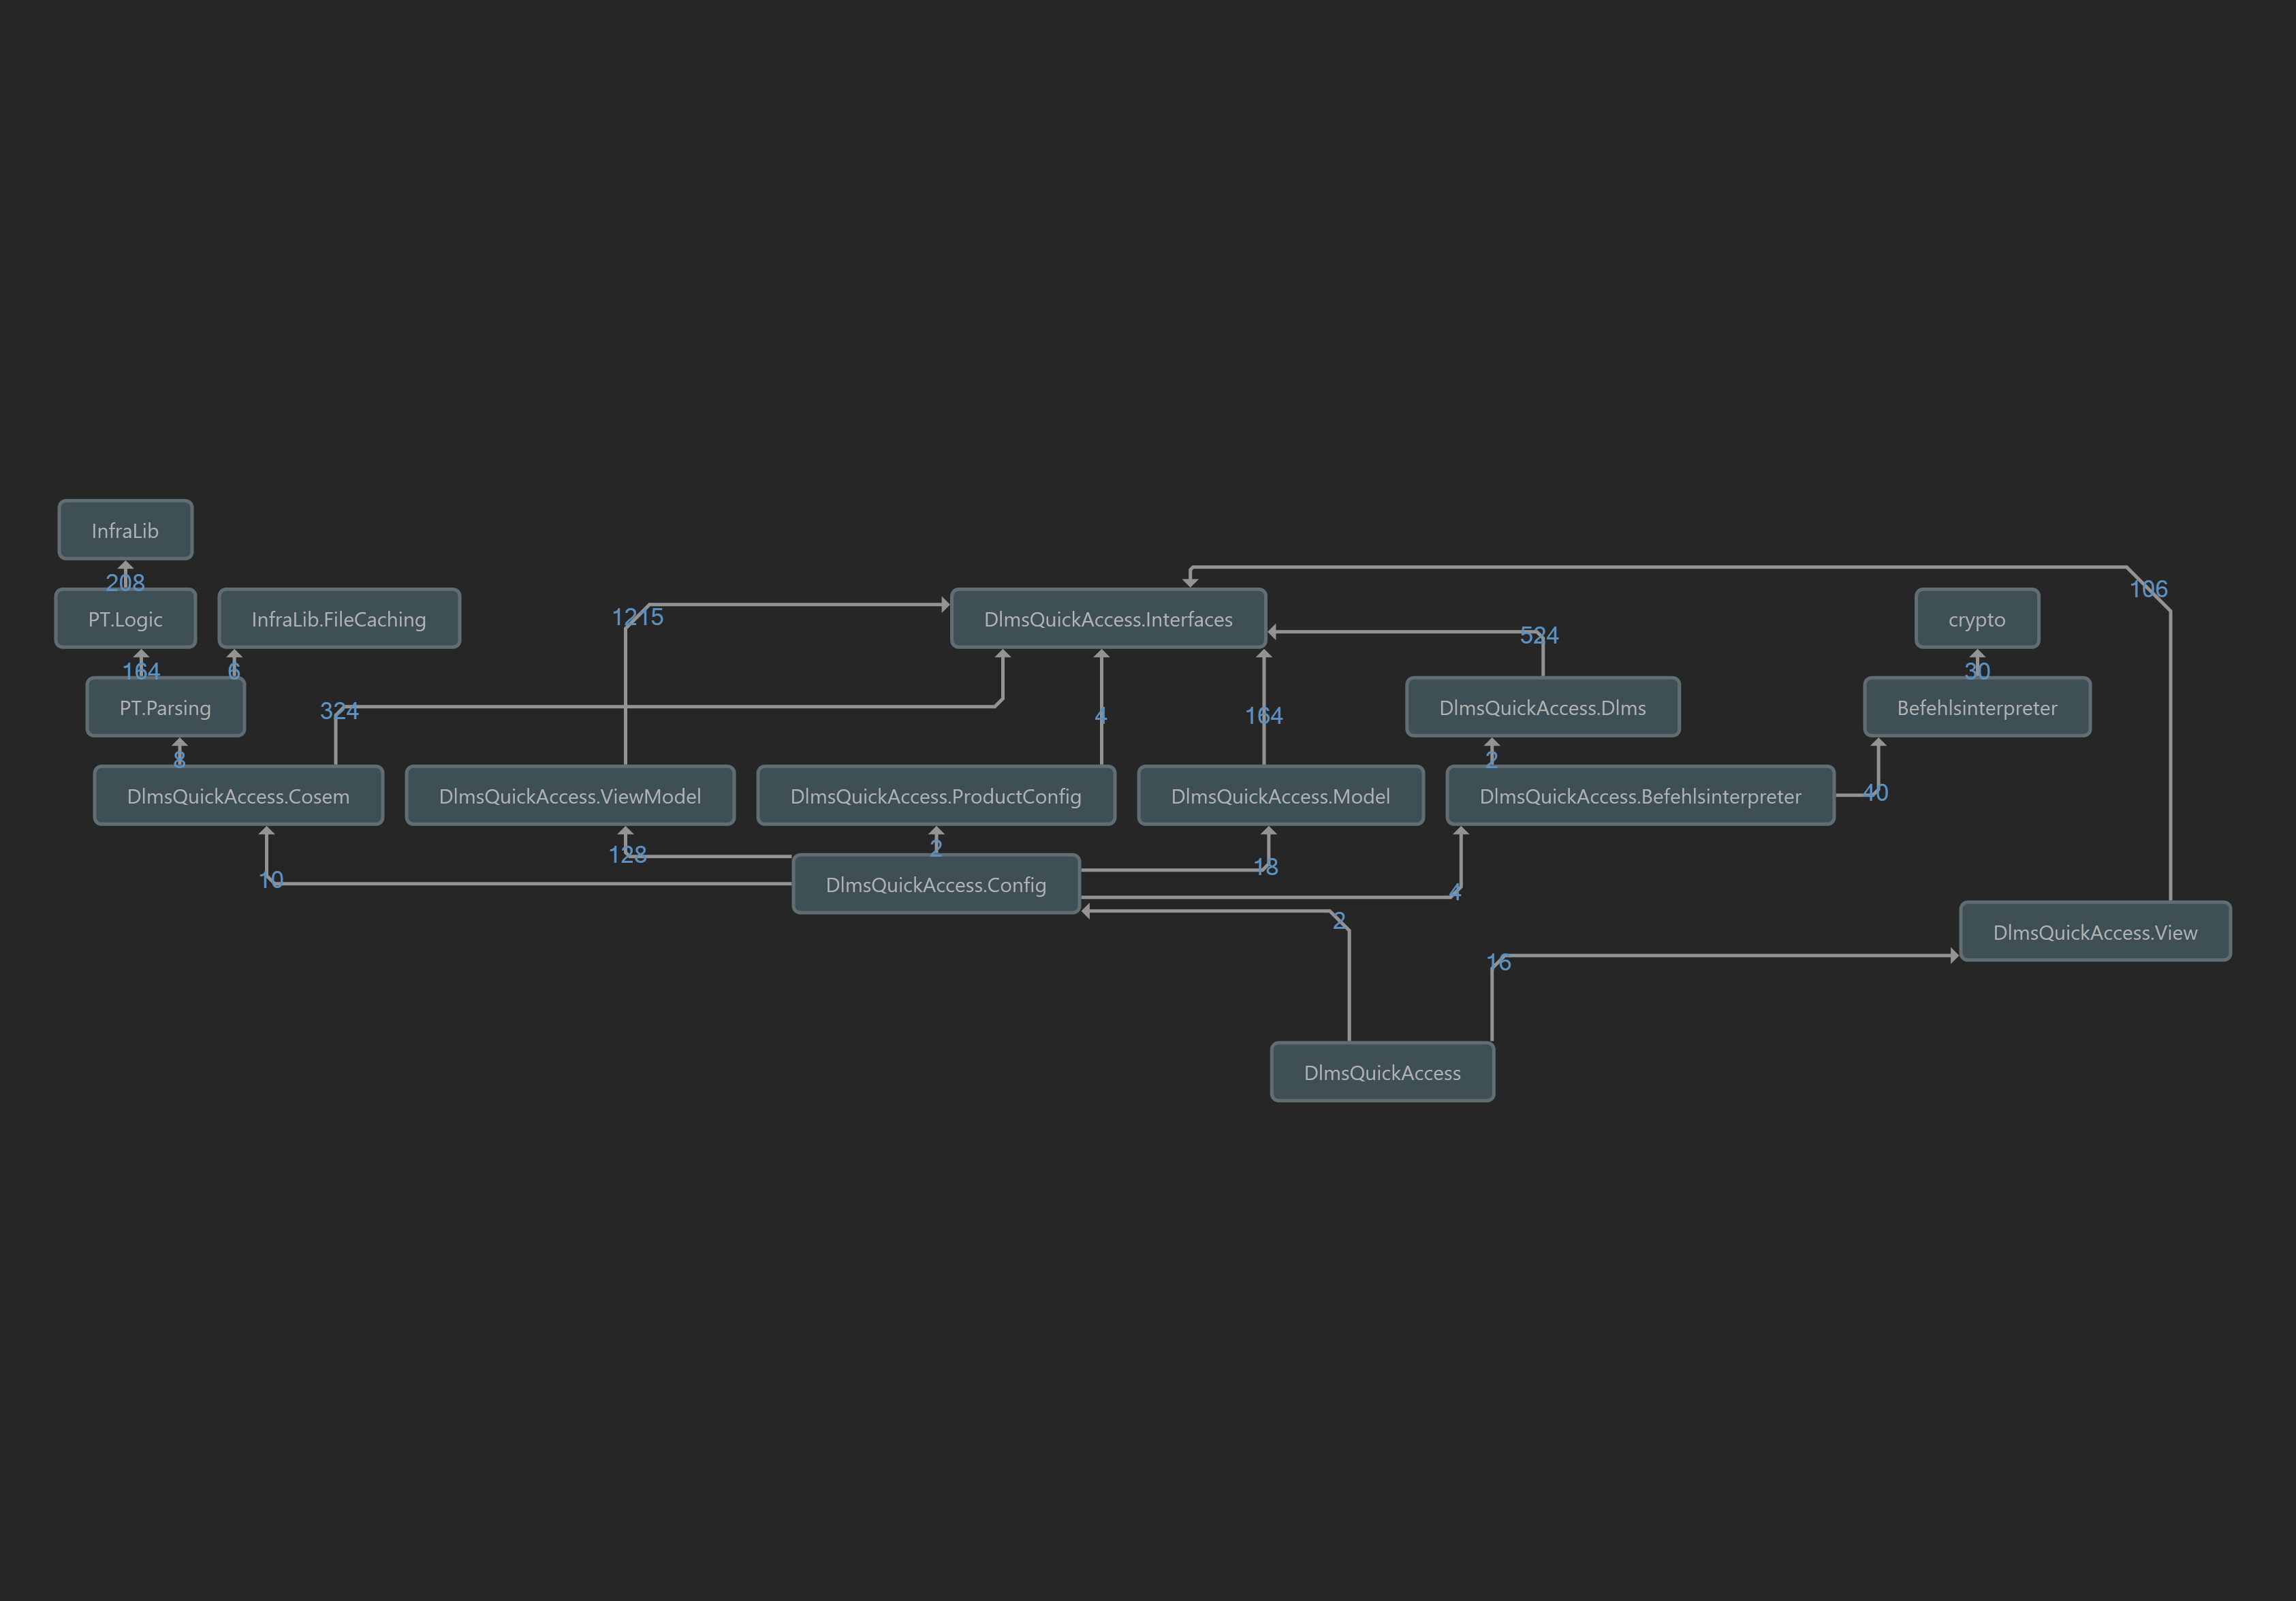
\includegraphics[width=1.0\textwidth]{gfx/Architecture view for DlmsQuickAccess.png}
   \caption{
      Abhänigkeiten der Projekte
   }
   \label{fig:projectDependencies}
\end{figure}

In der Abbildung \ref{fig:projectDependencies} sind alle Projekte und deren Abhängigkeit aufgezeigt.
Diese werden in den folgenden Abschnitten näher beschrieben.

\subsection{DlmsQuickAccess}
Dieses Projekt ist der Einstiegspunk der Anwendung.
Die Klasse \textit{App} lässt sich mit der \texttt{main()} Method vergleichen, welchen den meisten C basierten Sprachen als erstes ausgeführt, wenn ein Programm gestartet wird.
Diese lädt \textit{Windows} und \textit{Controls} aus dem DlmsQuickAccess.View Projekt und zeigt diese dem Nutzer an.


\subsection{DlmsQuickAccess.Config}

\subsection{DlmsQuickAccess.View}
Sämtliche Komponenten der Benutzerschnittstelle, also \textit{Windows} und \textit{Controls}, sind in diesem Projekt definiert. 
Nebst der Abhängigkeit zum Framework WinUI3, welches für die Darstellung der Element der Benutzerschnittstelle benötigt wird, gibt es nur eine einzige Abhängigkeit, jene zu DlmsQuickAccess.Interfaces.
Diese ist dazu da, dass die Controls die Interfaces der ViewModels kennen, auf welche sie binden.
Das Zusammenspiel von View und ViewModel ist im Abschnitt (\ref{mvvm}) beschrieben.
Währen diese Interfaces im selben Projekt wie die Controls definiert, so hätten die Implementationen der ViewModels eine Abhängigkeit auf DlmsQuickAccess.View.
Um eine solche Koppelung zu vermeiden, wurden die Interfaces in ein eigenes Projekt ausgelagert.


\subsection{DlmsQuickAccess.ViewModel}



\subsection{DlmsQuickAccess.Interfaces}

\subsection{DlmsQuickAccess.ProductConfig}
External dependency to yamllib


\subsection{DlmsQuickAccess.Dlms}
evtl widerverwendbar

\subsection{DlmsQuickAccess.Cosem}
evtl widerverwendbar
infralib etc.

\subsection{DlmsQuickAccess.Befehlsinterpreter}
isolation des Befehlsinterpreter



